\documentclass[journal, letterpaper]{IEEEtran}
%\documentclass{scrartcl}

\usepackage[ngerman,english]{babel}
%\usepackage[latin1]{inputenc}
\usepackage[utf8]{inputenc}
\usepackage[T1]{fontenc}
\usepackage{amsmath}
\usepackage{amsthm}
\usepackage{amsfonts}
\usepackage{tikz}
\usepackage{verbatim}
\usepackage{subcaption}
\usepackage{algorithm}
\usepackage{algorithmic}
\usepackage[pdftex]{hyperref}

\renewcommand{\algorithmicrequire}{\textbf{Input:}}
\renewcommand{\algorithmiccomment}[1]{\ \ // #1} % C-like // Comments

\hyphenation{render}

% No clubs and widows allowed
\clubpenalty10000
\widowpenalty10000
\displaywidowpenalty=10000

\begin{document}

%\title{Simulating elastic spheres without external forces}
%\subtitle{Project 1 for class CS6491 Computer Graphics}
\title{Swirl\\
	{\large Project 2 for class CS6491 Computer Graphics}}
%\author{Sebastian Weiss}
\author{Sebastian Weiss, Kristian Eberhardson\\ \today}
%\date{\today}

\maketitle

\begin{tikzpicture}[remember picture,overlay]
   \node[anchor=north east,inner sep=0pt] at (current page.north east)
              {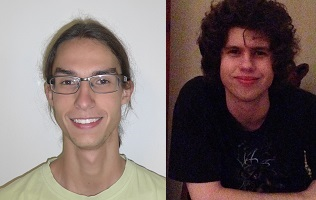
\includegraphics[scale=1]{pic}};
\end{tikzpicture}
\begin{tikzpicture}[remember picture,overlay]
   \node[anchor=north west,inner sep=10pt] at (current page.north west)
              {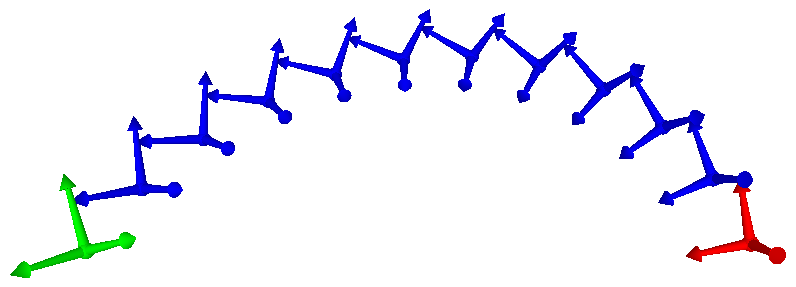
\includegraphics[scale=0.4]{pictures/P4.png}};
\end{tikzpicture}

\section{Objective}
We are provided with a starting and ending frame, called $A_0$ and $A_1$. We wish to create a continuous, affine and steady motion which interpolates $A_0$ and $A_1$.
 
\section{Input}
The Frames $A_0$ and $A_1$ consist of a point $P_i$ and a right hand coordinate system of orthogonal vectors $I_i$, $J_i$, and $K_i$, each of the same length ($i \in \{0,1\}$).
\subsection{Terms} 
1. An \underline{affine} transformation in three dimensions can be expressed as a 4x4 matrix multiplied onto a point or a vector, is reversible, and can be expressed solely as a combination of rotation, translation, and scaling.
\newline
2. A \underline{continuous} transformation is one in which $\forall \epsilon>0 \; \exists \delta>0 \; \text{s.th.} \; |P_x - P_y|<\epsilon \; \forall x,y \; \text{with} \; |x-y|<\delta$. $P_x$ and $P_y$ denotes the interpolated point at time $x$ and $y$. Intuitively, this means we can draw the motion with a pen in a single stroke.
\newline
3. A \underline{steady} transformation preserves the angle between a pair of frames, and is independent of some time t. 

\section{Related interpolation schemes}

\subsection{Logarithmic spiral in 2D}
In 2D, a frame is given by three two-dimensional vectors. Prof. Rossignac proposes a combination of a linear rotation and an exponential scaling to realize a steady interpolation between two dimensional frames, see Fig. \ref{fig:P6}.
The formula for this approach is the following:
\begin{equation}
 P(t) := F + m^t FP_0 ^{\;\circ} (\alpha t)
\label{eq:logSpiral}
\end{equation}
$FP_0 ^{\;\circ} (\alpha t)$ denotes the normal 2d rotation of the vector $FP_0$ around the origin with the angle $\alpha t$.
\begin{figure}[H]
	\centering
		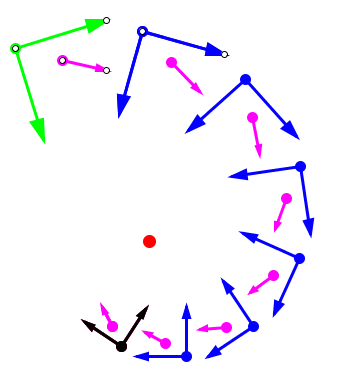
\includegraphics[scale=0.4]{pictures/P6.png}
	\caption{log spiral in 2D}
	\label{fig:P6}
\end{figure}

\subsection{Linear interpolation in 3D}
For all points in $A_0$, draw a straight line to its corresponding point in $A_1$. Motion is simply moving the frame along these lines.  This is neither an elegant solution nor does it preserve the area of the frame.

\section{Proposed model}
We wish to create a swirling motion in 3D related to the logarithmic spiral in 2D. Therefore, we are using a combination of linear rotation around the rotation axis $N$ with the origin in $F$ and an exponential scaling with the factor $m$. We propose the following formula:
\begin{equation}
 P(t) := F + m^t FP_0 ^{\;\circ} (\alpha t; N)
\label{eq:Interpolation}
\end{equation}
Since the rotation and scaling are steady on its own and these operations commute, the final motion is also steady.

\subsection{3D rotation}
A rotation in 2D is very straightforward because there is no choice of the rotation axis. In 3D we are given the rotation axis and rotate around it in the following way:

\begin{equation}
\begin{array}{lcl}
 X^{\circ}(\alpha; N) &:=& W + U^{\circ}(\alpha; N) \\
                        & =& W + \cos \alpha U - \sin \alpha (N \times U) \\
 \multicolumn{3}{l}{\text{with } W := W\angle\underline{N} = (W\bullet\underline{N})\underline{N}} \\
 \multicolumn{3}{l}{\text{and } U = X-W}
\end{array}
\label{eq:Rotation}
\end{equation}

Fig. \ref{tikz:Rot} visualizes the rotation around the axis $N$ in 3D.

\begin{figure}[H]
\centering
\begin{tikzpicture}
	\filldraw[color=white,fill=blue!20,fill opacity=0.5] (-3,-1.5) -- (2,-1.5) -- (3,1.5) -- (-2,1.5) -- cycle;
	\draw[color=orange] (-0.5,0) arc (-180:-61.7:0.5);
	\draw[line width=1mm,color=black!60,->] (0,0) -- (-1.5,0);
	\draw[line width=1mm,color=black!60,->] (0,0) -- (0.7,-1.3);
	\draw[line width=1mm,dotted,color=black!50] (-1.5,0) -- (-1.5,1);
	\draw[line width=1mm,dotted,color=black!50] (0.7,-1.3) -- (0.7,0.5);
	\draw[line width=1.5mm,color=green,->,line cap=round] (0,0) -- (-1.5,1);
	\draw[line width=1.5mm,color=red,->,line cap=round] (0,0) -- (0.7,0.5);
	\draw[line width=1.5mm,color=black,->,line cap=round] (0,0) -- (0,2);
	\node at (0.4,2) {$N$};
	\node at (-0.7,1) {$FP_0$};
	\node at (0.5,0.7) {$FP_1$};
	\node at (-1.8,0.5) {$W$};
	\node at (1,-0.4) {$W$};
	\node at (-0.75,-0.3) {$U$};
	\node at (0.1,-0.9) {$U$};
	\node[color=orange] at (-0.35,-0.6) {$\alpha$};
\end{tikzpicture}
\caption{3D-Rotation}
\label{tikz:Rot}
\end{figure}


\subsection{Calculating $N$, $\alpha$ and $m$}
Since $m$ is the scaling factor, it is calculated as:
\begin{equation}
 m := |I_1| / |I_0|
\label{eq:m}
\end{equation}
Because $I_i$, $J_i$, and $K_i$ are of the same length for each $i$, it does not matter which we use. 
 
To calculate the rotation axis $N$, we first define 
\begin{equation}
\Delta I:= I_1 - I_0, \ \Delta J := J_1 - J_0, \ \Delta K := K_1 - K_0
\end{equation}
Then we pick the largest vector in the euclidean norm out of 
\begin{equation}
N_a := \Delta I \times \Delta J, \ N_b := \Delta I \times \Delta K, \ N_c := \Delta J \times \Delta K
\end{equation}
We call the largest vector $N$. Since $I_i$, $J_i$ and $K_i$ form an orthogonal basis, these vectors all point in the same direction and differ only in the scaling. The reasons for choosing the largest one are numerically issues. Some of these $N$'s can be very small when the rotation axis is almost parallel to the frame axes, they are zero if they are exactly parallel. The special case when all $N$'s are zero, so $\Delta I$, $\Delta J$ and $\Delta K$ are all zero, happens if there is no rotation at all. See section \ref{NoRot} on how to deal with this case. In the later computation, we always need the normalized vector $\underline{N}:=N/|N|$.
  
Furthermore, we need the rotation angle $\alpha$. To compute this angle, we first project each basis vector into the plane defined by $\underline{N}$ and normalize them:
\begin{equation}
\begin{array}{lcl}
 proj(X) &:=& X - X\angle\underline{N} = X - (X \bullet \underline{N})\underline{N} \\
 norm(X) &:=& X / |X| \\
 B' &:=& norm(proj(B_i)) \ \forall B \in \{I_0,...,K_1\}
\end{array}
\label{eq:ProjBasis}
\end{equation}
The $B'$-vectors correspond to normalized versions of the $U$-vectors in Fig. \ref{tikz:Rot}.
Then we define
\begin{equation}
 \alpha = \max \{ \cos^{-1}(I_0' \bullet I_1'), \cos^{-1}(J_0' \bullet J_1'), \cos^{-1}(K_0' \bullet K_1') \}
\label{eq:}
\end{equation}
We take the maximum angle here because all angles are equal by the definition of $N$. At most one of these angles can be zero, this happens in the case if the rotation axis is exactly orthogonal to that frame axis, see Fig. \ref{fig:P1}.
\begin{figure}
	\centering
		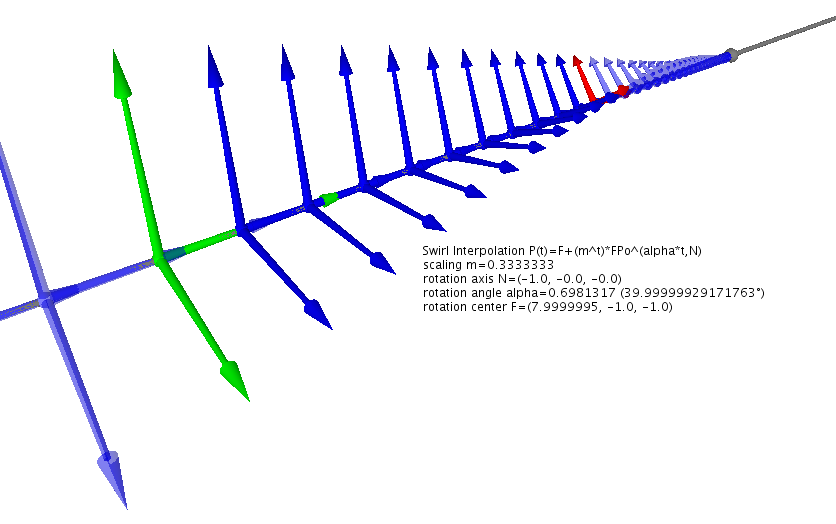
\includegraphics[scale=0.4]{pictures/P1.png}
	\caption{rotation parallel to a frame axis}
	\label{fig:P1}
\end{figure}

\subsection{Calculating $F$}
Now we have $N$, $\alpha$ and $m$ and we can compute $F$ now by solving the equation system
\begin{equation}
 P_1 = P(1) := F + m FP_0 ^{\;\circ} (\alpha; N)
\label{eq:Feq}
\end{equation}
This system is a linear system in the three variables $F_x$, $F_y$ and $F_z$. We obtain an explicit formulation for $F$ by converting it into matrix form, solving it using Cramer's Rule and applying simplification. For purposes of notation, we introduce the following variables for the vector components: $P_0=(P_{0,x},P_{0,y},P_{0,z})^T, P_1=(P_{1,x},P_{1,y},P_{1,z})^T,\\ \underline{N}=(N_x,N_y,N_z)^T$.
\begin{equation}
\begin{array}{lcl}
	F_x &=& (m P_{0,x} + m^3 P_{0,x} - P_{1,x} - m^2 P_{1,x} \\
		&& + m (1+m) (\cos\alpha - 1) (P_{0,x} - P_{1,x}) N_y^2 \\
		&& + m (1+m) (\cos\alpha - 1) (P_{0,x} - P_{1,x}) N_z^2 \\
		&& - m (1+m) (\cos\alpha - 1) (P_{0,y} - P_{1,y}) N_x N_y \\
		&& - m (1+m) (\cos\alpha - 1) (P_{0,z} - P_{1,z}) N_x N_z \\
		&& - m (m-1) \sin\alpha (P_{0,y} - P_{1,y}) N_z \\
		&& + m (m-1) \sin\alpha (P_{0,z} - P_{1,z}) N_y \\
		&& - 2 m^2 P_{0,x} \cos\alpha + 2 m P_{1,x} \cos\alpha ) \\
		&& / (m-1)(1 + m^2 - 2m\cos\alpha)
\end{array}
\label{eq:Fx}
\end{equation}
\begin{equation}
\begin{array}{lcl}
 F_y &=& -(m^2 P_{0,y} - m^3 P_{0,y} + P_{1,y} - m P_{1,y} \\
		&& + m (1+m) (\cos\alpha - 1) (P_{0,x} - P_{1,x}) N_x N_y \\
		&& + m (1+m) (\cos\alpha - 1) (P_{0,y} - P_{1,y}) N_y^2 \\
		&& + m (1+m) (\cos\alpha - 1) (P_{0,z} - P_{1,z}) N_y N_z \\
		&& - m (m-1) \sin\alpha (P_{0,x} - P_{1,x}) N_z \\
		&& + m (m-1) \sin\alpha (P_{0,z} - P_{1,z}) N_x \\
		&& - m P_{0,y} \cos\alpha + m^2 P_{0,y} \cos\alpha \\
		&& - m P_{1,y} \cos\alpha + m^2 P_{1,y} \cos\alpha) \\
		&& / (m-1)(1 + m^2 - 2m\cos\alpha)
\end{array}
\label{eq:Fy}
\end{equation}
\begin{equation}
\begin{array}{lcl}
 F_z &=& -(m^2 P_{0,z} - m^3 P_{0,z} + P_{1,z} - m P_{1,z} \\
		&& + m (1+m) (\cos\alpha - 1) (P_{0,x} - P_{1,x}) N_x N_z \\
		&& + m (1+m) (\cos\alpha - 1) (P_{0,y} - P_{1,y}) N_y N_z \\
		&& + m (1+m) (\cos\alpha - 1) (P_{0,z} - P_{1,z}) N_z^2 \\
		&& - m (m-1) \sin\alpha (P_{0,y} - P_{1,y}) N_x \\
		&& + m (m-1) \sin\alpha (P_{0,x} - P_{1,x}) N_y \\
		&& - m P_{0,z} \cos\alpha + m^2 P_{0,z} \cos\alpha \\
		&& - m P_{1,z} \cos\alpha + m^2 P_{1,z} \cos\alpha) \\
		&& / (m-1)(1 + m^2 - 2m\cos\alpha)
\end{array}
\label{eq:Fz}
\end{equation}
For the implementation, we strongly suggest to further factorize these formulas and to store the common intermediate results.

\subsection{Dealing with special cases}
The proposed model contains two singularities in the computations: 
First, $N$ is the zero vector when the rotation between the two input frames is zero.
Second, $F$ goes to infinity when $m$ goes to one, since the translation of the frames rely on the scaling.

\subsubsection{No rotation, but scaling}\label{NoRot}
In the case that there is no rotation, the rotation axis $N$ is the zero vector and the rotation angle $\alpha$ is also zero.
The translation is then realized by the scaling, see Fig. \ref{fig:P2}. The fixpoint $F$ is calculated as usual. Intuitively, this is the intersection point of the lines connecting the tips of the arrows and the frame origin from the start frame to the end frame.
\begin{figure}
	\centering
		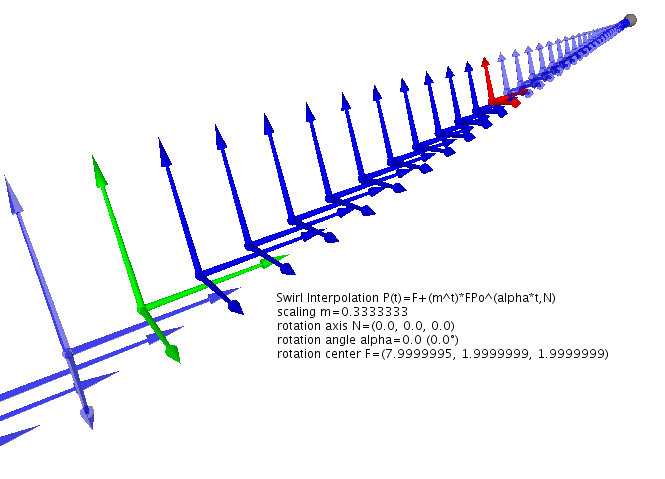
\includegraphics[scale=0.4]{pictures/P2.png}
	\caption{no rotation, translation by scaling}
	\label{fig:P2}
\end{figure}

\subsubsection{No rotation, no scaling}
If we start with the case presented in the previous section and let $m$ run to 1, the fixpoint $F$ runs against infinity. We therefore observe that the case of no rotation and no scaling degenerates to a linear interpolation with pure translation, see Fig. \ref{fig:P5}.
\begin{figure}
	\centering
		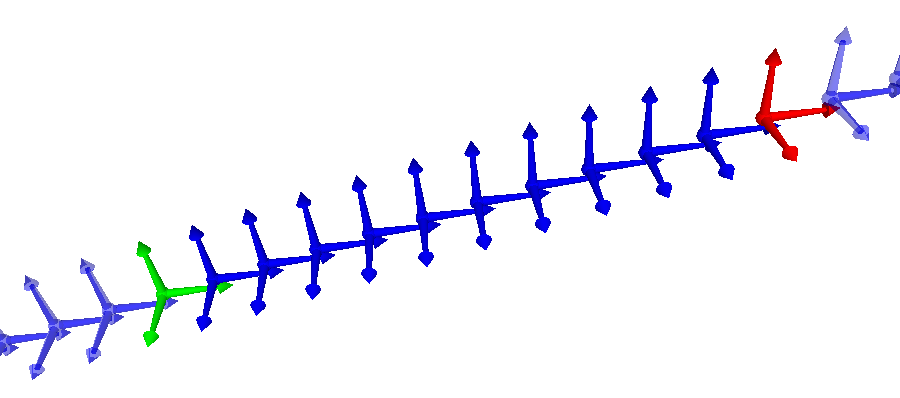
\includegraphics[scale=0.4]{pictures/P5.png}
	\caption{pure translation}
	\label{fig:P5}
\end{figure}

\subsubsection{No scaling, but rotation and translation}
If the scaling factor $m$ is 1, $F$ goes to infinity. The swirl degenerates to a circular movement in the rotation plane plus a linear translation orthogonal to the rotation plane. The swirl is therefore a perfect spiral, see Fig. \ref{fig:P7}.
\begin{figure}
	\centering
		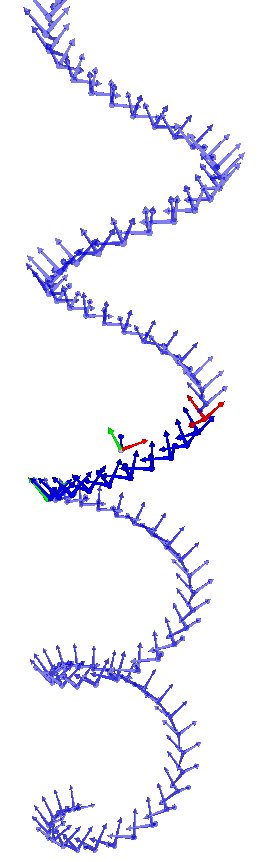
\includegraphics[scale=0.4]{pictures/P7.png}
	\caption{no scaling, but rotation and translation}
	\label{fig:P7}
\end{figure}
This special case can be implemented by projecting the frames in the rotation plane, solving the circular motion there equivalent to the Logarithmic Spiral in 2D and then adding a translation orthogonal to the rotation plane.

\section{Implementation}
We provide a framework for playing around with our Swirl Implementation. You can rotate the camera and scale it. Furthermore, the start and end frame can be modified by clicking and dragging the center of the frames or the tips of the frame axes. Additionally, you can select if you want to display the rotation axis $N$ (gray line) and the fixpoint $F$ (gray sphere on the rotation axis) and if the extrapolating frames should be drawn or not. 

A typical swirl produced by our program is shown in Fig. \ref{fig:P3}. You can see how the motion is attracted by the fixpoint $F$.

\begin{figure}
	\centering
		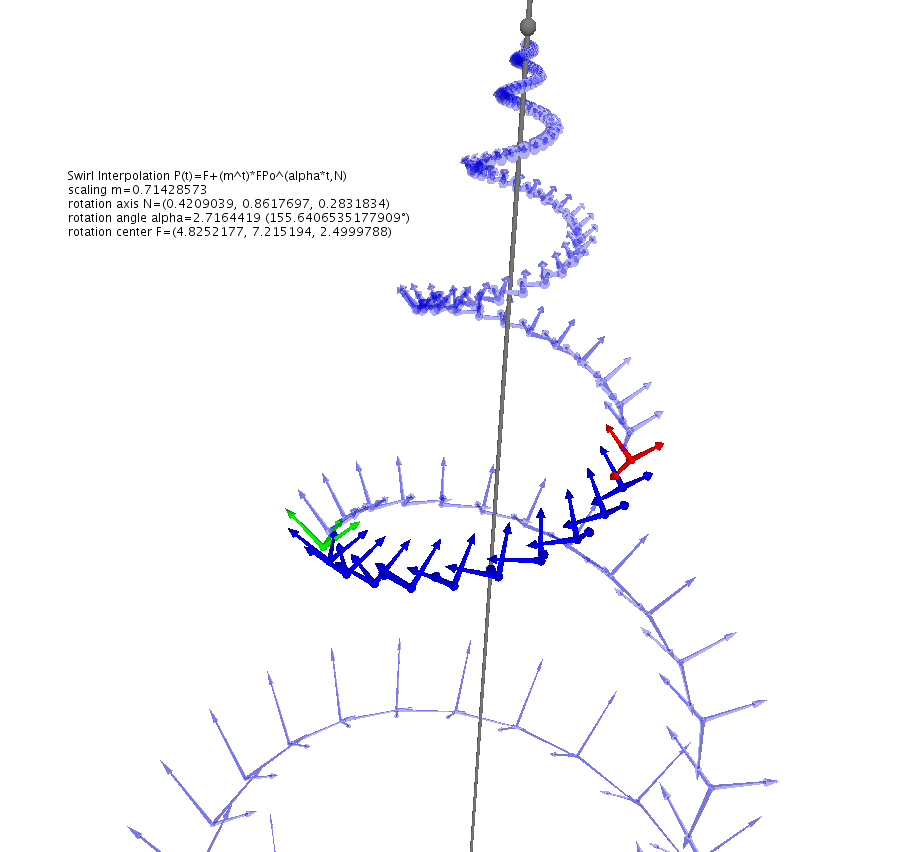
\includegraphics[scale=0.4]{pictures/P3.png}
	\caption{swirl motion is attracted by the fixpoint $F$}
	\label{fig:P3}
\end{figure}


\end{document}